\section{The role of the sequence length}
In this section, we focus on a first new emerging characteristic of the \emph{sequence single-index models} over the vanilla \emph{single-index models}: the sequence length \(L\). Therefore, we neglect the effect of the positional encoding, by setting \(P=0\), in order to isolate just the effect of the sequence length. The goal of the section is to measure the speed-up that a model like Equation~\eqref{2506:eq:model-definition} can achieve over the plain \emph{single-index models} when processing sequential data with length \(L\).

\paragraph{Linear attention ---} 
Our first goal is to understand the dependence of the convergence rate of SGD on the sequence length. For that, consider the particular case of \emph{linear attention}, given by the reduction map:
\begin{equation}
    \Pi[A] = \vec{a}_\mathrm{left}^\top A \vec{a}_\mathrm{right} \quad \text{with } \vec{a}_\mathrm{left} = \vec{a}_\mathrm{right} = \frac{1}{\sqrt{L}} \left(1, 1, \ldots, 1\right)^\top \in \mathbb{R}^L.
\end{equation}
Rearranging the terms
\begin{equation}
    f_{\vec{w}}(\vec{z}) = \vec{a}_\mathrm{left}^\top \left(\vec{z}\vec{z}^\top\right) \vec{a}_\mathrm{right} = \frac{1}{L} \sum_{i=1}^L \sum_{j=1}^L z_i z_j = \left(\sum_{i=1}^L \frac{z_i}{\sqrt{L}}\right)^2 = \left(\frac{\Flatten(X)\cdot \vec{w}_\mathrm{tied}}{\sqrt{L}}\right)^2,
\end{equation}
where \(\vec{w}_\mathrm{tied} \coloneqq \mathrm{concat}(\vec{w}, \dots, \vec{w}) \in \mathbb{R}^{Ld}\) is the concatenation of \(L\) copies of \(\vec{w}\). This model is equivalent to a \emph{generalized linear model} with \emph{tied weights}, and activation function \(\sigma(x) = x^2\). In terms of performance, taking a general activation \(\sigma\) will at worst be the same as the \emph{attention mechanism} originally considered, if not better. More precisely, we consider:
\begin{equation} \label{2506:eq:tied-network-definition}
    f_{\vec{w}}(X) = \sigma\left(\frac{\Flatten(X)\cdot \vec{w}_\mathrm{tied}}{\sqrt{L}}\right).
\end{equation}
This is the most generic model we study in this section. Further numerical experiments elucidating the equivalence of the speed-up for this \emph{tied network} and for the attention models can be found in Appendix~\ref{2506:app:further-sequence-length}. Note that \emph{tied networks} are not restricted to learn even functions only, differently from the model in Equation~\eqref{2506:eq:model-definition}.

\paragraph{The corresponding untied network ---} Given the model in Equation~\eqref{2506:eq:tied-network-definition}, a natural benchmark is the model with untied weights. Let \(W \in \mathbb{R}^{L\times d}\) be the matrix of weights, whose rows are all updated with Equation~\eqref{2506:eq:normalized-SGD-w}, the untied network is given by
\begin{equation} \label{2506:eq:untied-network-definition}
    f_{W}(X) = \sigma\left(\frac{\Flatten(X)\cdot \Flatten(W)}{\sqrt{L}}\right).
\end{equation}
Since we have \(L\) independent weights (the rows of \(W\)) the sufficient statistic measuring the overlap between the model and the target SSI is not a scalar as for the tied network, but a vector of length \(L\)
\begin{equation}
    \vec{m} = \frac{W\vec{w}_\star}{d} \in \mathbb{R}^L \quad\text{compacted to a scalar as}\quad m_\mathrm{untied} = \frac{\norm{\vec{m}} }{\sqrt{L}}.
\end{equation}

% % \paragraph{Beyond the sample complexity} A part from pathological choices of \(y^\mathrm{SSI}\) (see Appendix~\ref{2506:app:further-sequence-length}, the sample complexity of SGD is the same for both tied and untied networks. However, the scaling of \(\nu^\mathrm{weak}_\eta\) with \(L\) can sensibly change depending on the particular target. We need a result that could characterize precisely this scaling for the weak recovery.
% % \begin{theorem}[Informal] \label{2506:thm:ode}
% %     Let \(y^\mathrm{SSI}\) be a target function with sequence information exponent $\sie$, to be learned with an tied network.
% %     Assume the activation function \(\sigma\) has a sufficiently rich Hermite expansion such that it matches the leading order of the \(y^\mathrm{SIE}\),  Then the overlap $m(t)$ of the solution to \eqref{2506:eq:ode_approx} before weak recovery is well approximated by the solution \(\bar{m}(t)\) of the following ODE
% %     \begin{equation} \label{2506:eq:ode-at-initialization-tied}
% %         \dod{m}{t} = \alpha(L) m^{\mathrm{SIE}-1} - \frac{\gamma}{2}\beta(L) m.
% %     \end{equation}
% %     \(\alpha(L)\) and \(\beta(L)\) are two functions of \(L\) and depends on \(\sigma\) and the target \(y^\mathrm{SSI}\).
% % \end{theorem}
% % The explicit expression of \(\alpha(L)\) and \(\beta(L)\), as well as the formal statement of the Theorem, and the proof can be found in Appendix~\ref{2506:app:proofs}. Equation~\eqref{2506:eq:ode-at-initialization-tied} is the leading order approximation of the \emph{Saad\&Solla equation} of the system \cite{saad1995line}.
% % An equivalent result holds for the untied network, where \(\alpha\) and \(\beta\) are replaced by \(\alpha_\mathrm{untied}(L)\) and \(\beta_\mathrm{untied}(L)\); the details are in Appendix~\ref{2506:app:proofs}. 

\paragraph{Measuring the speed-up ---}
The learning rate plays an important role in determining the number of gradient steps needed to reach weak recovery: the larger the learning rate \(\gamma(L)\) is, the faster the model learns. However, if it becomes too large, SGD will fail to converge, never achieving weak recovery. The gradient-flow approximation in Equation~\eqref{2506:eq:ode_approx} exhibits this effect: when \(\gamma\) becomes too large the dynamic of the system is not attracted by \(\vec{w}_\star\) or \(P\) anymore, and there is no learning. In order to have a faithful measure of the speed-up, we will assume that the learning rate is taken to be the largest possible that guarantees weak recovery; we discuss this upper bound on the learning rate in Appendix~\ref{2506:app:further-sequence-length}.

We measure the speed-up of tied networks with respect to untied networks, as measured in terms of number of gradient steps needed to reach weak recovery, by the ratio of the weak recovery times in the two cases
\begin{equation}
    \mathrm{gain}(L)  \coloneqq \frac{\nu^\mathrm{weak}_{\eta,\mathrm{untied}}}{\nu^\mathrm{weak}_\eta},
\end{equation}
where \(\nu^\mathrm{weak}_{\eta,\mathrm{untied}}\) is given by Definition~\ref{2506:def:weak-recovery} where \(m\) is replaced by \(m_\mathrm{untied}\); the dependence of \(\mathrm{gain}\) on \(\eta\) is subleading, and we will neglect it in the following. 

\begin{theorem} \label{2506:thm:sequencelength-gain}
    Let $C_{\sie} \in \dR^{L^\sie}$ be the first non-zero tensor in the Hermite expansion of $g$ (see Appendix~\ref{2506:app:hermite-polynomials}). Then the gain satisfies with high probability
    \[ \mathrm{gain} \gtrsim \left(\frac{C_{\sie} \times (\mathbf{1}, \dots, \mathbf{1})}{\norm{C_\sie}_{\mathrm{op}}}\right)^2 \cdot \begin{cases}
        L & \text{if } \sie = 1 \\
        1 & \text{otherwise}
    \end{cases}. \]
    If the tensor $C_{\sie}$ is \emph{orthogonally decomposable}, in particular in the cases where $\sie \leq 2$ or $g$ is separable, then
    \[ \mathrm{gain} \asymp \left(\frac{C_{\sie} \times (\mathbf{1}, \dots, \mathbf{1})}{\norm{C_\sie}_{\mathrm{op}}}\right)^2\cdot \begin{cases}
        L & \text{if } \sie = 1 \\
        1 & \text{otherwise}
    \end{cases}. \]
\end{theorem}
By definition of the operator norm, we have 
\[ C_{\sie} \times (\mathbf{1}, \dots, \mathbf{1}) \leq \norm{C_\sie}_{\mathrm{op}} L^{\sie/2},
\quad\text{and hence}\quad
0 \leq \mathrm{gain} \lesssim L^{\sie \vee 2}.\]
Since the untied network has \(L\) times the number of parameters compared to the tied one, a naive parameter counting argument would yield a \(\mathrm{gain}=L^{(SIE-1) \vee 1}\) expected gain. Counter-intuitively, the actual gain of using a tied network can either exceed or fall short of this naive value, depending on the function $g$. In pathological cases (see Appendix~\ref{2506:app:further-sequence-length}), the tied network can even either fail to learn the target, or do so slower than its untied counterpart.

\paragraph{Example for ${\rm SIE}=2$ ---}
Let's assume to have a target function \(g(\vec{z}_\star)= \sum_{i=1}^L \mathrm{He}_2(z_{\star,i})\). In this case, the SIE is \(2\) and the tensor \(C_2\) is simply the identity matrix \(I_L\). The gain is by
\[
    \mathrm{gain} \asymp \left(\frac{I_L \times (\mathbf{1}, \dots, \mathbf{1})}{\norm{I_L}_{\mathrm{op}}}\right)^2 \cdot 1 = \left(\frac{L}{1}\right)^2 \cdot 1 = L^2.
\]
\begin{figure}
    \centering
    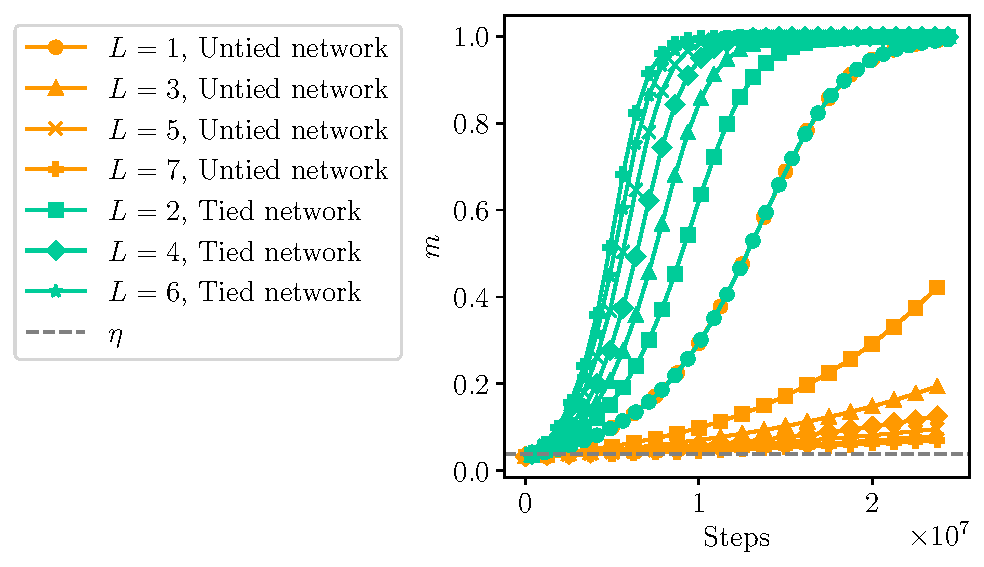
\includegraphics[height=0.37\textwidth]{figs/sequence-lenght/H2overlapevolution}
    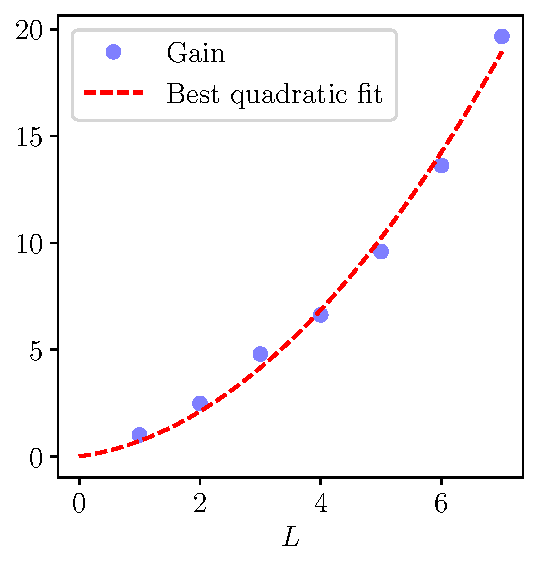
\includegraphics[height=0.37\textwidth]{figs/sequence-lenght/H2gain}
    \caption{Left: overlap \(m\) for tied (green) and untied (orange) networks as a function of the number of gradient steps; different symbols represent different values of \(L\).
    Right: measured gain as a function of the sequence length \(L\), with the best fit line showing its scaling as \(L^2\). \(g(\vec{z}_\star)= \sum_{i=1}^L \mathrm{He}_2(z_{\star,i})\), \(d=1000\), \(\sigma = \ReLU\).}
    \label{2506:fig:sequence-length-H2}
\end{figure}
Figure~\ref{2506:fig:sequence-length-H2} show a numerical experiment, with a \(\ReLU\) activation, confirming the result of Theorem~\ref{2506:thm:sequencelength-gain}.
